\documentclass{llncs}

\usepackage{graphicx}
\usepackage{a4wide}
\usepackage{url}



\title{Nao as a RoboTutor}
\author{Anass Drif \and Hans Gaiser \and Jethro Tan \and Pim Veldhuisen \and Koen V. Hindriks}
\institute{Delft University of Technology}

%
%
%
\begin{document}

\maketitle

\begin{abstract}
The aim of the RoboTutor project is to develop a Nao robot that is able to educate and entertain an audience. Key challenges are to maintain audience attention and to interact with the audience. As a first step towards this goal, a system has been developed that enables the Nao to present a lecture on robotics with a focus on itself as an example of a humanoid robot. The system enables a Nao to present, explain, and control a slide show and to dynamically change slides while presenting. Moreover, during the presentation the Nao interacts with its audience in various ways to keep them engaged and entertained by performing quizzes and demonstrating some of its capabilities.
\end{abstract}

%
%
\section{Introduction}
What comes to mind when you think about education? Chances are that it involves an experienced teacher talking to a number of students. But why is this the most common way of teaching? In most cases all of the concepts the teacher is conveying are also available in books, explaining them cleary, concisely and at the student's own pace. Still, most students choose to listen to a teacher instead of reading a book, even when attendance is optional. Why? Beacuse teaching is so much more than saying words. Teaching is about interaction, about asking questions, about humor; about connecting with the audience.\\

The world of education is changing through new technologies. Massive open online courses are very popular these days, with renowned institutions joining the pioneers. These courses are a great way to reach large audiences, but often lack interaction. Here lies an opportunity for robots, who could provide embodied interaction with an audience. However, interaction is not easy to achieve for robots. A lot of research exist on interaction between robots and single humans, but research on interaction between robots and audiences is scarce. The NAO robot has mainly been used for one-on-one interaction with human beings. In entertainment however, the main goal is to have one-to-many interaction, similar to the interaction between teacher and students. The practical goal of the Robotutor project is to develop a robot lecturer, that can assist a professor with his lectures. The academic benefits of this project are twofold: research is done in the field of one-to-many interaction and the project itself is a very insightful process in which it is necessary to reflect on the question what really is important in education.



%
%
\section{Virtual Teachers}\label{sec:virtual}
The deployment of virtual teacher could provide many advantages over their human counterparts. In line with other applications for virtual agents, greater cost efficiency and availability can be used to either decrease expenditures or inprove utility. Focussing or the later, virtual teachers could more easily give a certain lecture at multiple timeslots or repeat and elaborate lectures for students having trouble understanding certain concepts.\\

Another great opportunity lies in the optimization of education. Virtual teachers could deliver the same lessons consistenly in great quantaties. The effects of minor changes in these lessons can thus be measured more reliably than in human teachers, where there is an natural variation in every instance that makes it hard to determine the effect of a change without taking in to account other differences. Expanding on this concept, machine learning for robotic teachers might even be envisaged. When the virtual agents recieve feedback on there performace, such as audience scores or even test results, the teachers could attempt to improve themselves in teaching there subject material. If the gathered information is shared across many teachers, this could lead to a self optimizing system of education. 

%
%
\section{Embodied Robots}\label{sec:embodied}
When opting for the use of modern technologies in education the choice for embodied robotics is not immediately obvious. Teaching tools such as videos, presentations, readings and quizzes can all be delivered through the familiar and readily available channel of the internet onto computers. Even when choosing for a solution that involves some form artificial intelligence, an abstract delivery system seems the most obvious choice. Although an experience involving embodied robotics is often more costly both in terms of money and effort, the greater cost can be amply offset by the benefits of embodiment.\\

Research show that embodied characters can increase performance of interacting subjects. \cite{Bartneck2002} This is most likely due to an increased level of social presence, motivating the people involved to put in more effort. Other studies show that embodied interaction is also experienced as more enjoyable, both in entertainment \cite{Pereira2008} and cognitive situations.\cite{Tapus2009}

These advantages are essential in educational situations and thus make the use of embodied agents preferable to virtual agents.



%
%
\section{Aldebaran's NAO robot}\label{sec:NAO}
The RoboTutor project uses the NAO robot from Aldebaran Technologies as it's embodied agent. The NAO is a humanoid robot with a height of 58 cm. It's size and shape make the NAO suitable for the role of teacher. It is likeable and open, but also makes a serious inpression. Its humanoid looks facilitates social engagement but avoids the uncanny valley effect.\cite{mori1970uncanny}\\

\begin{figure}
\centering
	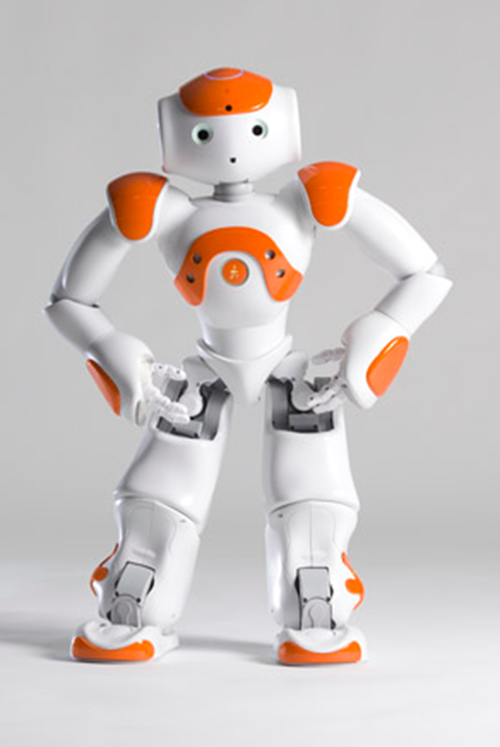
\includegraphics[scale=0.3]{images/NAO.png}
	\caption{The NAO robot}\label{fig:nao}
\end{figure}


The NAO is an out-of-the-box solution that comes with is own hardware. This means no hardware or firmware needs to be developed, allowing for a focus on higher hierarchical layers. This forms a limitation in adaptability, but the NAO provides great flexibility and fills all hardware requirements of the project. \\

The NAO has a flexible body with 25 degrees of freedom that allows it to move naturally and support its communication by body language. It also monitors its 37 sensors that allow it to respond to its audience and surroundings.\\




%
%
\section{RoboTutor System Architecture}\label{sec:architecture}
\subsection{Architecture}
The Robotutor's presentations are based on scripts. These are human made files containing the text of the presentation. This text is synthesized to speech by the NAO's engine during the presentation. Additionally the text also contains a number of commands. These are actions the robot will perform during the lecture, such as its movements. The pacing of the slideshow is also controlled using these commands.\\
During the presentation, two pieces of software facilitate the execution of the script. The first part runs on the computer that is used for the presentation. This computer is connected to the beamer or screen and runs the slideshow. Another part runs on the NAO, controlling the execution of the script, the speech synthesis and the robot's behaviour.\\

The application executed on the computer that runs the slideshow is created using the Qt-toolkit, which is a graphical toolkit written in C++ and is commonly used for cross platform applications. Through this application the user can control the Robotutor application running on the robot. These controls include connecting to the robot, running a script, pausing a script and stopping a script. When this application is launched, it will automatically also launch a Powerpoint instance with which it maintains a communication link. This allows the application to control the Powerpoint application, by for example triggering a next slide event or even adding slides. When the user closes the application, the Powerpoint application is also automatically closed. In addition, this application contains a simple text editor which the user can use to create a script. This text editor has some simple highlighting to indicate which parts are text that the NAO will speak out, which parts are behaviours the NAO will perform and which parts have been commented out and will be ignored.\

When the user decides it is time to start the script, the script is sent to the robot. The application running on the robot receives this message in plain text and interprets the script to determine what to do. For this purpose a custom script parser has been written in C++, which executes the script in real time. Blocks of text are send to the speech engine running on the NAO and the commands are being handled in the appropriate ways. In the case of a command to run a behaviour, it is added to a queue and will be executed when the speech engine notifies it is time for that behaviour to be executed. Commands to change a slide are send back to the computer side when it is time to execute them. The computer side then forwards this to Powerpoint.\

The two applications talk to each other through a protocol called Google Protocol Buffers. Protocol buffers is a method to serialize structured data to allow for easy sending over a network channel. In this case it is used to send a script or commands from one application to the other. The use of  Google Protocol Buffers provides a language-neutral, platform-neutral, extensible way to send the required data. \

\begin{figure}
	\includegraphics[scale=0.1]{images/system_overview_sober.png}
	\caption{A schematic overview of the system. Red arrows indicate control flow, black arrows indicate data flow.}
\end{figure}

\subsection{Special Features}
\subsubsection{Powerpoint}
The robot can go to the next slide, step back or forward a specific number of slides, or go to a certain slide. Additionally, slides with new content can be dynamically created.

\subsubsection{Turningpoint}
The Turningpoint system consists of a number of response cards, small electronic devices, connected to a computer. The response card are handed out to people in the audience, who can use them to digitally respond to a question. Turningpoint then aggregates and presents the results. This can be used by a lecturer to check the audiences opinon or knowledge. The use of this technology is integrated into the Robotutor system. Using it, the NAO can ask questions and interpret the results. This provides a great method for interaction with the audience.
The system can also be used to present a choice to the audience. For example, the robot could ask is a certain concept is clear to the audience or is more explanation is necessary. Here the robot could again make a decision based on the results.\\

Turningpoint questions are started by a command in the script. The script engine then asks the local engine to initiate a Turningpoint session through Powerpoint. When the polling is done, the local engine reads an XML-file containing the results of the quiz. The results of the quiz are then send to the script engine, which then decides what to do with them.

\subsubsection{Pulse Audio}
In large rooms or lecture halls, the NAO's internal speakers might not have enough volume to serve the audience properly. For these kind of situations audio streaming has been implemented. Using pulse audio, the NAO's sound can be redirected to a different set of speakers.

\subsubsection{Taking Pictures}
A command is available to take a picture using one of the NAO's cameras. This picture is then displayed on a new Powerpoint slide. This usually means the audience can see itself, creating a humorous moment, but also confirming that the presentation is happening in real time.

\subsubsection{Teacher Interruption}
At any moment the teacher can pause the execution of the script using the graphical interface or by touching the head of the NAO.

\subsubsection{Noise level}
The system can monitor the noise level in the room, and respond accordingly if there is too much noise. Additionally the noise level can be visualized live on a Powerpoint slide.



%
%
\section{Preliminary Evaluation}\label{sec:evaluation}
One finding during early trials of the system was that the robot needs to be continuously moving because otherwise attention of the audience drops. This poses several technical challenges again. First, the motors of the joints can overheat. In our case, we can actually use such motor ``failure" to explain something about the workings of the robot joints. Second, we found that the robot cannot simply perform random gestures but the timing and type of gestures displayed should make sense and match the spoken text.

The RoboTutor has been put to the test in front of a real audience a number of times throughout its development. The duration of the lecture presentations varied from about five to twenty minutes. In general we have been surprised by the robot's ability to capture audience attention and to convey information. This was true even though we used the out-of-the-box synthesized voice of the Nao robot with almost no modifications; participants in our initial try-outs agreed that the robot's voice does not pose a big problem. 

During the demonstrations the quizzes turned out to be a great source of interaction. The questions asked by the Nao trigger the audience to think about what the robot said and to use the information provided in the lecture. But more importantly the response of the RoboTutor to the answers received from the audience shows that the RoboTutor is able to interact with its audience, and, as a result, the audience feels engaged. In addition it provides a tool to evaluate and analyse knowledge transfer from the RoboTutor to its audience and to study how to effective educate an audience.

It appears also quite important that the robot somehow conveys that it is aware of its audience. Simple mechanisms could enhance the feeling of robot awareness in its audience. For example, the robot could look at and point more explicitly to the slides during the presentation and then look back at audience. This type of behaviour would help suggest that the robot is aware of where it is looking at. It also remains a challenge to make the robot appear to look more or less randomly at participants in its audience and thus improve the feeling that the robot is aware of its audience. The robot could also be made to appear more situation-aware by including a simple event-based mechanism that allows the robot to await for an event and to respond to an event.


%
%
\section{Conclusion}\label{sec:conclusion}
The RoboTutor system enables a Nao to interact with an audience in an engaging way. In initial trials the RoboTutor was able to maintain audience attention and receive positive feedback. The system can also be used in other settings and, for example, be used as a quiz master.



%
%
\section{Future Work}\label{sec:future}
The RoboTutor is promising but a lot of work remains to be done to develop more engaging and interactive robotic tutors. An important aspect of this development would be the realisation of a system for beter sensing of the audience. One prospective way of doing this would be the use of an advanced vision system (possibly in combination with an external camera). Such a system would allow the RoboTutor to increase its spatial awareness, by enabling it to locate the teacher and individuals in its audience. Moreover, the robot could monitor the audience and respond to it. For example, by seeing a raised hand the RoboTutor might detect that a student in the classroom wants to ask a question. Ofcourse it is then imperative the robot can also respond to this event and allow the student to speak. This would mean the script that the robot follows needs to be interrupted at certain times. To facilitate this, a control layer would be needed to coordinate the alternation between the script and audience events. Last but not least, after allowing the student to speak, the RoboTutor should also be able to respond to the inquiry. This would require integrating advanced state-of-the-art question answering systems.

%
%
\bibliographystyle{splncs}
\bibliography{references}


\end{document}